\documentclass[]{article}
\usepackage{lmodern}
\usepackage{amssymb,amsmath}
\usepackage{ifxetex,ifluatex}
\usepackage{fixltx2e} % provides \textsubscript
\ifnum 0\ifxetex 1\fi\ifluatex 1\fi=0 % if pdftex
  \usepackage[T1]{fontenc}
  \usepackage[utf8]{inputenc}
\else % if luatex or xelatex
  \ifxetex
    \usepackage{mathspec}
  \else
    \usepackage{fontspec}
  \fi
  \defaultfontfeatures{Ligatures=TeX,Scale=MatchLowercase}
\fi
% use upquote if available, for straight quotes in verbatim environments
\IfFileExists{upquote.sty}{\usepackage{upquote}}{}
% use microtype if available
\IfFileExists{microtype.sty}{%
\usepackage{microtype}
\UseMicrotypeSet[protrusion]{basicmath} % disable protrusion for tt fonts
}{}
\usepackage[margin=1in]{geometry}
\usepackage{hyperref}
\hypersetup{unicode=true,
            pdftitle={36-315 Homework 02, Spring 2019},
            pdfauthor={Eu Jing Chua},
            pdfborder={0 0 0},
            breaklinks=true}
\urlstyle{same}  % don't use monospace font for urls
\usepackage{color}
\usepackage{fancyvrb}
\newcommand{\VerbBar}{|}
\newcommand{\VERB}{\Verb[commandchars=\\\{\}]}
\DefineVerbatimEnvironment{Highlighting}{Verbatim}{commandchars=\\\{\}}
% Add ',fontsize=\small' for more characters per line
\usepackage{framed}
\definecolor{shadecolor}{RGB}{248,248,248}
\newenvironment{Shaded}{\begin{snugshade}}{\end{snugshade}}
\newcommand{\AlertTok}[1]{\textcolor[rgb]{0.94,0.16,0.16}{#1}}
\newcommand{\AnnotationTok}[1]{\textcolor[rgb]{0.56,0.35,0.01}{\textbf{\textit{#1}}}}
\newcommand{\AttributeTok}[1]{\textcolor[rgb]{0.77,0.63,0.00}{#1}}
\newcommand{\BaseNTok}[1]{\textcolor[rgb]{0.00,0.00,0.81}{#1}}
\newcommand{\BuiltInTok}[1]{#1}
\newcommand{\CharTok}[1]{\textcolor[rgb]{0.31,0.60,0.02}{#1}}
\newcommand{\CommentTok}[1]{\textcolor[rgb]{0.56,0.35,0.01}{\textit{#1}}}
\newcommand{\CommentVarTok}[1]{\textcolor[rgb]{0.56,0.35,0.01}{\textbf{\textit{#1}}}}
\newcommand{\ConstantTok}[1]{\textcolor[rgb]{0.00,0.00,0.00}{#1}}
\newcommand{\ControlFlowTok}[1]{\textcolor[rgb]{0.13,0.29,0.53}{\textbf{#1}}}
\newcommand{\DataTypeTok}[1]{\textcolor[rgb]{0.13,0.29,0.53}{#1}}
\newcommand{\DecValTok}[1]{\textcolor[rgb]{0.00,0.00,0.81}{#1}}
\newcommand{\DocumentationTok}[1]{\textcolor[rgb]{0.56,0.35,0.01}{\textbf{\textit{#1}}}}
\newcommand{\ErrorTok}[1]{\textcolor[rgb]{0.64,0.00,0.00}{\textbf{#1}}}
\newcommand{\ExtensionTok}[1]{#1}
\newcommand{\FloatTok}[1]{\textcolor[rgb]{0.00,0.00,0.81}{#1}}
\newcommand{\FunctionTok}[1]{\textcolor[rgb]{0.00,0.00,0.00}{#1}}
\newcommand{\ImportTok}[1]{#1}
\newcommand{\InformationTok}[1]{\textcolor[rgb]{0.56,0.35,0.01}{\textbf{\textit{#1}}}}
\newcommand{\KeywordTok}[1]{\textcolor[rgb]{0.13,0.29,0.53}{\textbf{#1}}}
\newcommand{\NormalTok}[1]{#1}
\newcommand{\OperatorTok}[1]{\textcolor[rgb]{0.81,0.36,0.00}{\textbf{#1}}}
\newcommand{\OtherTok}[1]{\textcolor[rgb]{0.56,0.35,0.01}{#1}}
\newcommand{\PreprocessorTok}[1]{\textcolor[rgb]{0.56,0.35,0.01}{\textit{#1}}}
\newcommand{\RegionMarkerTok}[1]{#1}
\newcommand{\SpecialCharTok}[1]{\textcolor[rgb]{0.00,0.00,0.00}{#1}}
\newcommand{\SpecialStringTok}[1]{\textcolor[rgb]{0.31,0.60,0.02}{#1}}
\newcommand{\StringTok}[1]{\textcolor[rgb]{0.31,0.60,0.02}{#1}}
\newcommand{\VariableTok}[1]{\textcolor[rgb]{0.00,0.00,0.00}{#1}}
\newcommand{\VerbatimStringTok}[1]{\textcolor[rgb]{0.31,0.60,0.02}{#1}}
\newcommand{\WarningTok}[1]{\textcolor[rgb]{0.56,0.35,0.01}{\textbf{\textit{#1}}}}
\usepackage{graphicx,grffile}
\makeatletter
\def\maxwidth{\ifdim\Gin@nat@width>\linewidth\linewidth\else\Gin@nat@width\fi}
\def\maxheight{\ifdim\Gin@nat@height>\textheight\textheight\else\Gin@nat@height\fi}
\makeatother
% Scale images if necessary, so that they will not overflow the page
% margins by default, and it is still possible to overwrite the defaults
% using explicit options in \includegraphics[width, height, ...]{}
\setkeys{Gin}{width=\maxwidth,height=\maxheight,keepaspectratio}
\IfFileExists{parskip.sty}{%
\usepackage{parskip}
}{% else
\setlength{\parindent}{0pt}
\setlength{\parskip}{6pt plus 2pt minus 1pt}
}
\setlength{\emergencystretch}{3em}  % prevent overfull lines
\providecommand{\tightlist}{%
  \setlength{\itemsep}{0pt}\setlength{\parskip}{0pt}}
\setcounter{secnumdepth}{0}
% Redefines (sub)paragraphs to behave more like sections
\ifx\paragraph\undefined\else
\let\oldparagraph\paragraph
\renewcommand{\paragraph}[1]{\oldparagraph{#1}\mbox{}}
\fi
\ifx\subparagraph\undefined\else
\let\oldsubparagraph\subparagraph
\renewcommand{\subparagraph}[1]{\oldsubparagraph{#1}\mbox{}}
\fi

%%% Use protect on footnotes to avoid problems with footnotes in titles
\let\rmarkdownfootnote\footnote%
\def\footnote{\protect\rmarkdownfootnote}

%%% Change title format to be more compact
\usepackage{titling}

% Create subtitle command for use in maketitle
\providecommand{\subtitle}[1]{
  \posttitle{
    \begin{center}\large#1\end{center}
    }
}

\setlength{\droptitle}{-2em}

  \title{36-315 Homework 02, Spring 2019}
    \pretitle{\vspace{\droptitle}\centering\huge}
  \posttitle{\par}
    \author{Eu Jing Chua}
    \preauthor{\centering\large\emph}
  \postauthor{\par}
      \predate{\centering\large\emph}
  \postdate{\par}
    \date{Due Wednesday, Sept 11, 2019 (11:59pm ET) on Canvas}


\begin{document}
\maketitle

\hypertarget{homework-02-introduction-to-ggplot-and-1-d-categorical-data}{%
\section{\texorpdfstring{Homework 02: Introduction to \texttt{ggplot}
and 1-D Categorical
Data}{Homework 02: Introduction to ggplot and 1-D Categorical Data}}\label{homework-02-introduction-to-ggplot-and-1-d-categorical-data}}

\begin{center}\rule{0.5\linewidth}{\linethickness}\end{center}

\begin{center}\rule{0.5\linewidth}{\linethickness}\end{center}

\hypertarget{problem-1}{%
\section{Problem 1}\label{problem-1}}

\textbf{\texttt{R} Style Guides: Google vs.~Hadley}:

\begin{enumerate}
\def\labelenumi{\alph{enumi}.}
\tightlist
\item
  (9 points) What are the main differences between these two style
  guides? Find at least 5 differences.
\end{enumerate}

\begin{itemize}
\tightlist
\item
  Google prefers using \texttt{BigCamelCase} for function names but
  Hadley prefers \texttt{lower\_snake\_case}.
\item
  Private functions should begin with a dot for Google
\item
  Google prefers explicit returns
\item
  Google does not support using right-hand assignment
\item
  Google also does not recommend using \texttt{attach()}
\end{itemize}

\begin{enumerate}
\def\labelenumi{\alph{enumi}.}
\setcounter{enumi}{1}
\tightlist
\item
  (1 point) Specify which style guide you will be using in this
  assignment.
\end{enumerate}

I will be using Hadley Wickham's style guide.

\begin{center}\rule{0.5\linewidth}{\linethickness}\end{center}

\begin{center}\rule{0.5\linewidth}{\linethickness}\end{center}

\hypertarget{problem-2}{%
\section{Problem 2}\label{problem-2}}

\textbf{Critiquing Graphs}:

\begin{enumerate}
\def\labelenumi{\alph{enumi}.}
\tightlist
\item
  (5 points) \textbf{Include the graph in your assignment}. Two choices
  here:
\end{enumerate}

\includegraphics{https://i.redd.it/o9elncd0xdk31.png}

\begin{enumerate}
\def\labelenumi{\alph{enumi}.}
\setcounter{enumi}{1}
\tightlist
\item
  (5 points) \textbf{Describe the graph}.
\end{enumerate}

The graph shows the proportion of each blood type in the US as a
pie-chart. The big labels indicate the general blood type letter (A, B,
AB, O) while the light and dark shading incidates the +/- of the blood
type. The main thing we can infer is that A+ and O+ dominates the
proportions.

\begin{enumerate}
\def\labelenumi{\alph{enumi}.}
\setcounter{enumi}{2}
\tightlist
\item
  (5 points) \textbf{Critique the graph}.
\end{enumerate}

The graph achieves its goal of showing the relative proportions of each
blood type in the US. It is very minimalistic in that there is no
unnecessary amount of data ink. However, there are no numerical labels
anywhere so we do not know the actual proportions, if the area of each
part of the pie-chart is proportional to the actual proportion. The
attempt at overlaping the blood type letter over two regions and using
color shades to differentiate the + and - succintly labels the regions,
but is abit too vague and requires additional interpretation. A color
map, showing the mapping between actual colors and blood types, would
help with this. Also, I would label the actual numerical proportions so
relative comparisons will be even easier and more accurate.

\begin{enumerate}
\def\labelenumi{\alph{enumi}.}
\setcounter{enumi}{3}
\tightlist
\item
  (5 points) \textbf{Critique the caption and/or surrounding text}.
\end{enumerate}

There is no surrounding text and captions, besides the main title
itself. The title is quite informative for this simple dataset and
nothing much else is needed. If anything, I think including some simple
information about which blood types can transfer to which others will
provide even more insight about what the distribution says about the
state of blood transfusions in the US.

\begin{center}\rule{0.5\linewidth}{\linethickness}\end{center}

\begin{center}\rule{0.5\linewidth}{\linethickness}\end{center}

\hypertarget{problem-3}{%
\section{Problem 3}\label{problem-3}}

\textbf{Bar Charts}:

\begin{enumerate}
\def\labelenumi{\alph{enumi}.}
\tightlist
\item
  (1 point) Load the Titanic data from Lab 02. How many rows does the
  dataset have? How many columns does the dataset have? Make sure that
  the variable \texttt{Pclass} is correctly recognized as
  \texttt{factor} variable by running
  \texttt{titanic\ \textless{}-\ mutate(titanic,\ Pclass\ =\ factor(Pclass))}
  if necessary. Is this an ordered variable?
\end{enumerate}

\begin{Shaded}
\begin{Highlighting}[]
\KeywordTok{library}\NormalTok{(tidyverse)}

\CommentTok{#  Load the data into R}
\NormalTok{titanic <-}\StringTok{ }\KeywordTok{read_csv}\NormalTok{(}\StringTok{"https://raw.githubusercontent.com/mateyneykov/315_code_data/master/data/titanic.csv"}\NormalTok{)}
\NormalTok{titanic <-}\StringTok{ }\KeywordTok{mutate}\NormalTok{(titanic, }\DataTypeTok{Pclass =} \KeywordTok{factor}\NormalTok{(Pclass))}

\KeywordTok{dim}\NormalTok{(titanic)}
\end{Highlighting}
\end{Shaded}

\begin{verbatim}
## [1] 712  12
\end{verbatim}

There are 712 rows and 12 columns. \texttt{Pclass} is not ordered as it
represents the ticket class, which has no inherent ordering (assume in
this case).

\begin{enumerate}
\def\labelenumi{\alph{enumi}.}
\setcounter{enumi}{1}
\tightlist
\item
  (5 points) Create a bar chart of the \texttt{Pclass} variable. Be that
  your axes are properly labeled, and that the graph has a proper title.
  Make sure that each bar in the graph has the same color. To do this,
  use \texttt{+\ geom\_bar(fill\ =\ "pink",\ color\ =\ "black")}. Change
  the \texttt{fill} and \texttt{color} commands. What do each of them
  do?
\end{enumerate}

\begin{Shaded}
\begin{Highlighting}[]
\KeywordTok{ggplot}\NormalTok{(titanic, }\KeywordTok{aes}\NormalTok{(}\DataTypeTok{x =}\NormalTok{ Pclass)) }\OperatorTok{+}
\StringTok{    }\KeywordTok{geom_bar}\NormalTok{(}\DataTypeTok{fill =} \StringTok{"lightblue"}\NormalTok{, }\DataTypeTok{color =} \StringTok{"black"}\NormalTok{) }\OperatorTok{+}
\StringTok{    }\KeywordTok{labs}\NormalTok{(}\DataTypeTok{title =} \StringTok{"Counts of Each Ticket Class"}\NormalTok{,}
         \DataTypeTok{x =} \StringTok{"Ticket Class"}\NormalTok{,}
         \DataTypeTok{y =} \StringTok{"Count"}\NormalTok{)}
\end{Highlighting}
\end{Shaded}

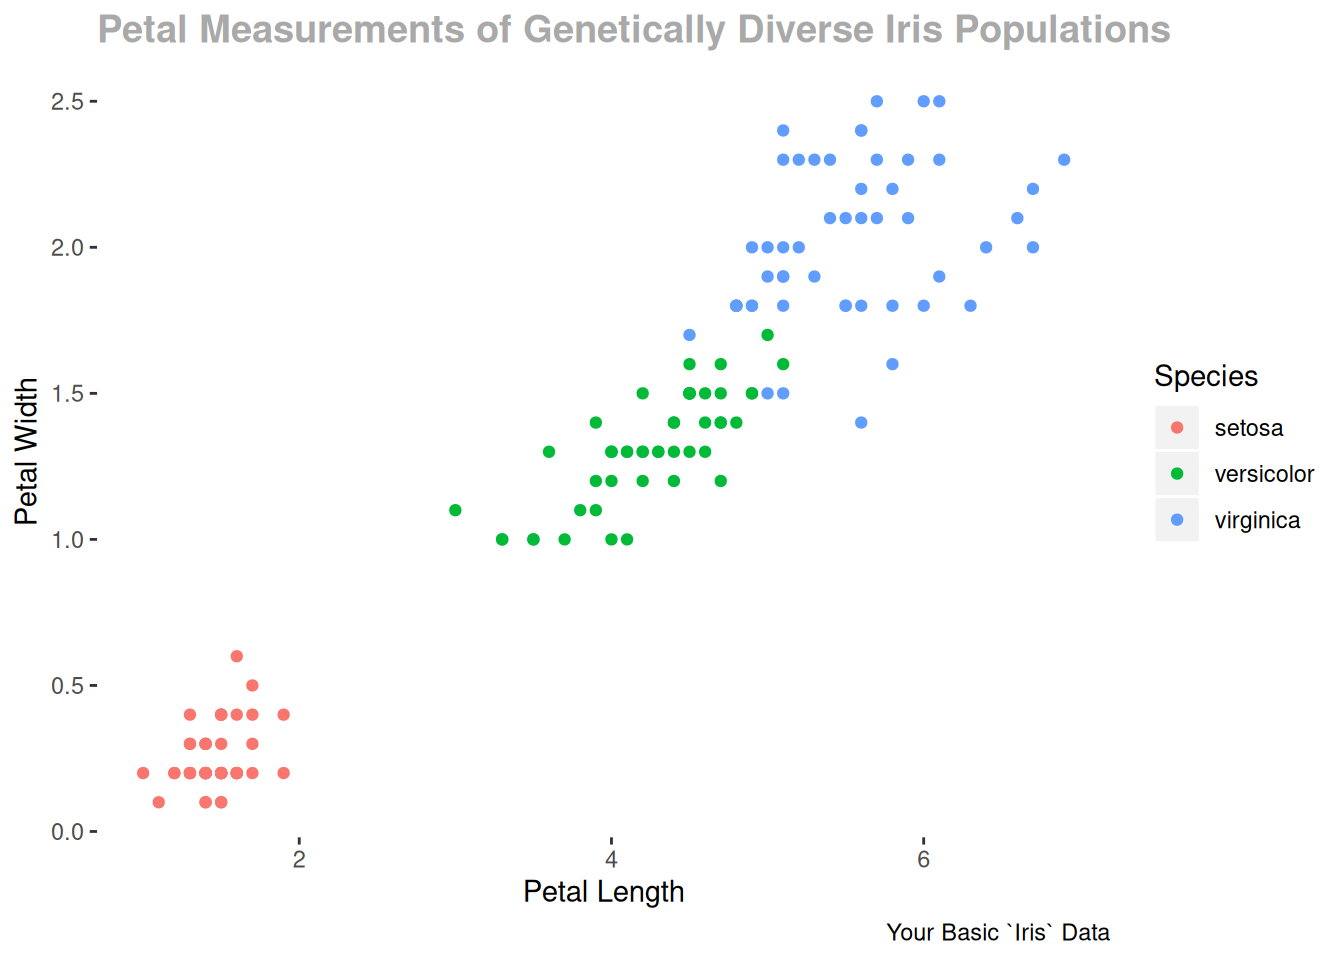
\includegraphics{Homework02_files/figure-latex/unnamed-chunk-2-1.pdf}

The \texttt{fill} changes the colors of the bars itself, and
\texttt{color} changes the color of the outline.

\begin{enumerate}
\def\labelenumi{\alph{enumi}.}
\setcounter{enumi}{2}
\tightlist
\item
  (4 points) You can also specify HEX color values when choosing a
  color, e.g.~\texttt{fill\ =\ "\#4169E1"}. Use a website like
  \href{http://www.w3schools.com/colors/colors_picker.asp}{this one} to
  pick a color of your choice, and fill the bars with that color (and
  display the updated graphic below).
\end{enumerate}

\begin{Shaded}
\begin{Highlighting}[]
\KeywordTok{ggplot}\NormalTok{(titanic, }\KeywordTok{aes}\NormalTok{(}\DataTypeTok{x =}\NormalTok{ Pclass)) }\OperatorTok{+}
\StringTok{    }\KeywordTok{geom_bar}\NormalTok{(}\DataTypeTok{fill =} \StringTok{"#4169E1"}\NormalTok{, }\DataTypeTok{color =} \StringTok{"black"}\NormalTok{) }\OperatorTok{+}
\StringTok{    }\KeywordTok{labs}\NormalTok{(}\DataTypeTok{title =} \StringTok{"Counts of Each Ticket Class"}\NormalTok{,}
         \DataTypeTok{x =} \StringTok{"Ticket Class"}\NormalTok{,}
         \DataTypeTok{y =} \StringTok{"Count"}\NormalTok{)}
\end{Highlighting}
\end{Shaded}

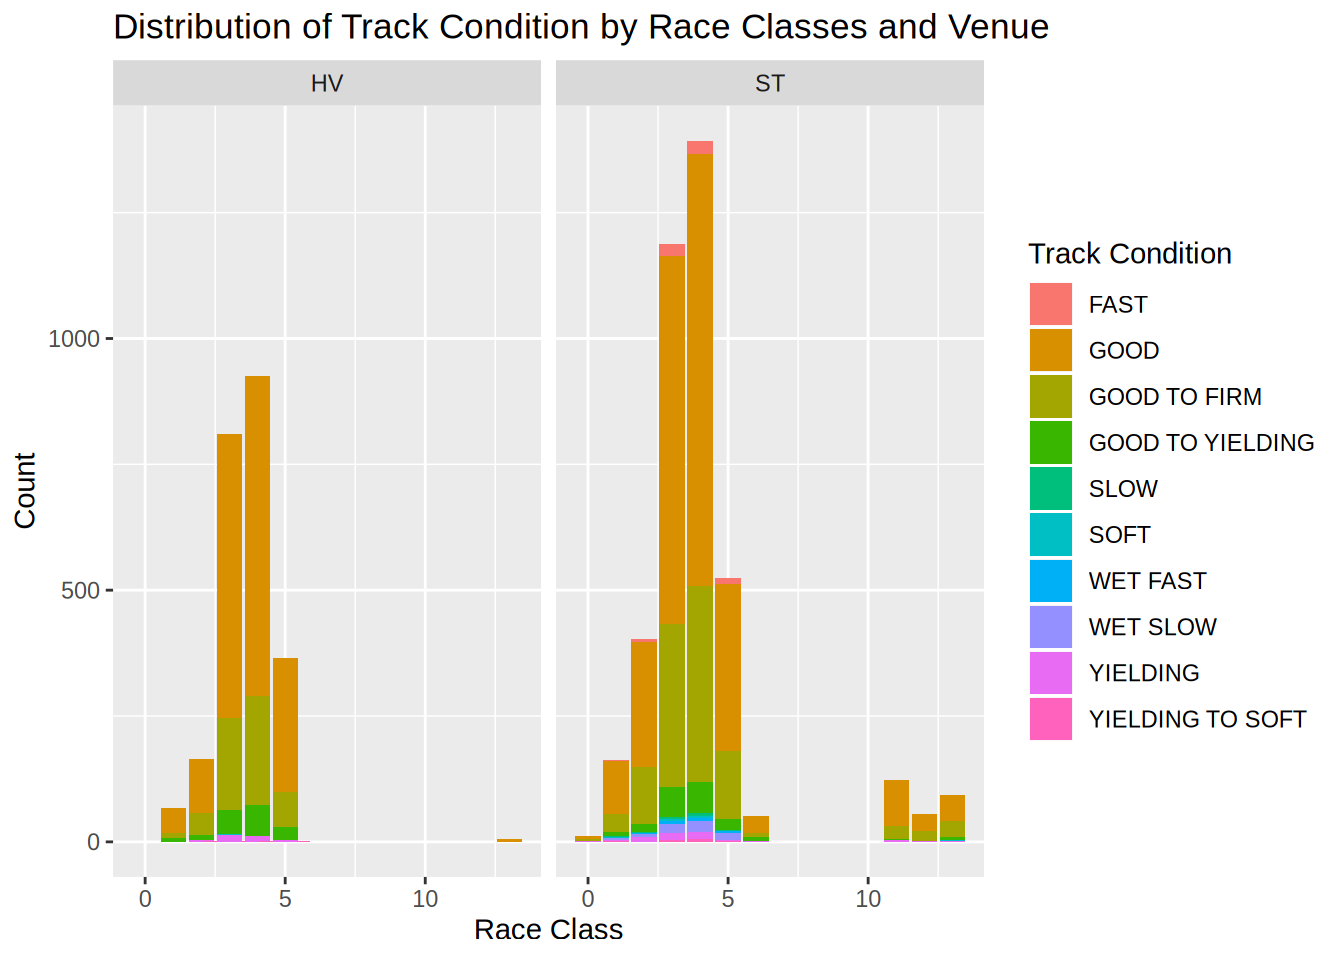
\includegraphics{Homework02_files/figure-latex/unnamed-chunk-3-1.pdf}

\begin{center}\rule{0.5\linewidth}{\linethickness}\end{center}

\begin{center}\rule{0.5\linewidth}{\linethickness}\end{center}

\hypertarget{problem-4}{%
\section{Problem 4}\label{problem-4}}

\textbf{Spine Charts}:

Spine Charts are similar to Bar Charts.

With a spine chart, we have a single (vertical) bar and multiple
stacked, horizontal bars. To do this, change the aesthetic arguments in
the \texttt{aes()} function in \texttt{geom\_bar()}. , e.g.:
\texttt{aes(x\ =\ factor(1),\ fill\ =\ my\_variable)}

This will create a single bar on the x-axis (since \texttt{factor(1)}
creates a one-category categorical variable of length one) and fill the
bar in with colors corresponding to whatever categorical values are in
\texttt{my\_variable}.

\begin{enumerate}
\def\labelenumi{\alph{enumi}.}
\tightlist
\item
  (4 points) Re-create the graph from Problem 3, but use a spine chart.
  That is, use a spine chart to show the distribution of
  \texttt{Pclass}. Be sure to correctly label the axes -- remember,
  their interpretation may have changed from Problem 3. Include an
  appropriate title (always do this).
\end{enumerate}

\begin{Shaded}
\begin{Highlighting}[]
\KeywordTok{ggplot}\NormalTok{(titanic, }\KeywordTok{aes}\NormalTok{(}\DataTypeTok{x =}\NormalTok{ Pclass)) }\OperatorTok{+}
\StringTok{    }\KeywordTok{geom_bar}\NormalTok{(}\KeywordTok{aes}\NormalTok{(}\DataTypeTok{x =} \KeywordTok{factor}\NormalTok{(}\DecValTok{1}\NormalTok{), }\DataTypeTok{fill =}\NormalTok{ Pclass), }\DataTypeTok{color =} \StringTok{"black"}\NormalTok{) }\OperatorTok{+}
\StringTok{    }\KeywordTok{labs}\NormalTok{(}\DataTypeTok{title =} \StringTok{"Counts of Each Ticket Class"}\NormalTok{,}
         \DataTypeTok{fill =} \StringTok{"Ticket Class"}\NormalTok{,}
         \DataTypeTok{x =} \StringTok{"Ticket Classes"}\NormalTok{,}
         \DataTypeTok{y =} \StringTok{"Proportions of Each Ticket Class"}\NormalTok{)}
\end{Highlighting}
\end{Shaded}

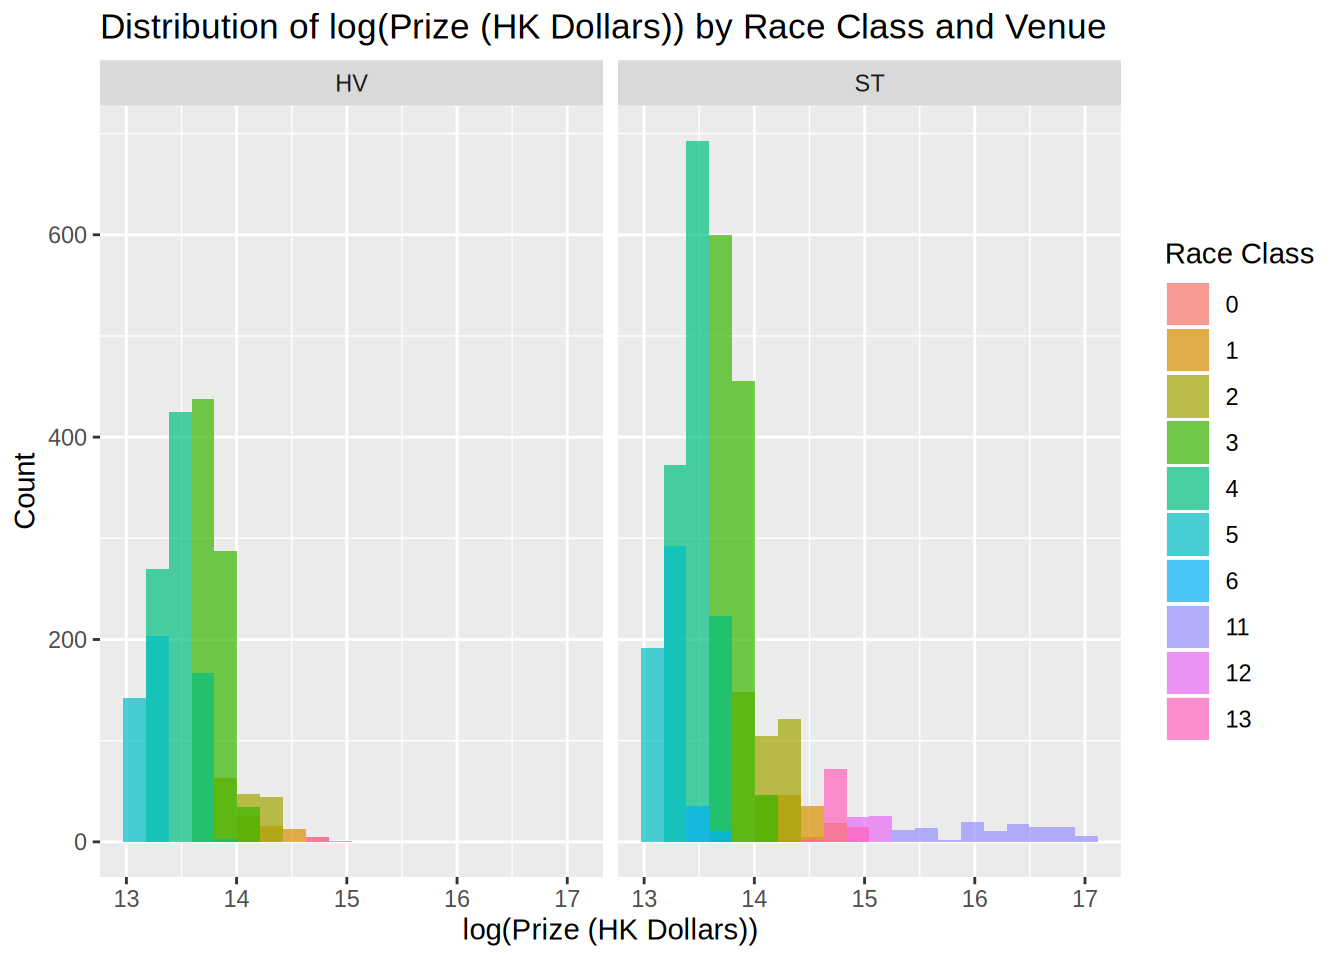
\includegraphics{Homework02_files/figure-latex/unnamed-chunk-4-1.pdf}

\begin{enumerate}
\def\labelenumi{\alph{enumi}.}
\setcounter{enumi}{1}
\tightlist
\item
  (3 points) In a spine chart, what are the widths of the bars
  proportional to (if anything)? What are the heights of the bars
  proportional to (if anything)? How is this different from a bar chart?
\end{enumerate}

In a spine chart, all widths are the same and thus are not proportional
to anything in particular. The heights of each component are
proportional to the counts we observe. In a bar chart, the bars are
separate and the height of each bar is the one proportional to the
counts we observe.

\begin{enumerate}
\def\labelenumi{\alph{enumi}.}
\setcounter{enumi}{2}
\tightlist
\item
  (3 points) \texttt{ggplot()} allows us to easily flip the orientation
  of our graphs without changing any of the code. To do this, you simply
  have to add \texttt{+\ coord\_flip()} to your existing code. Do this
  in a separate code block for the spine chart from part (a), and
  discuss the differences in the two plots.
\end{enumerate}

\begin{Shaded}
\begin{Highlighting}[]
\KeywordTok{ggplot}\NormalTok{(titanic, }\KeywordTok{aes}\NormalTok{(}\DataTypeTok{x =}\NormalTok{ Pclass)) }\OperatorTok{+}
\StringTok{    }\KeywordTok{geom_bar}\NormalTok{(}\KeywordTok{aes}\NormalTok{(}\DataTypeTok{x =} \KeywordTok{factor}\NormalTok{(}\DecValTok{1}\NormalTok{), }\DataTypeTok{fill =}\NormalTok{ Pclass), }\DataTypeTok{color =} \StringTok{"black"}\NormalTok{) }\OperatorTok{+}
\StringTok{    }\KeywordTok{labs}\NormalTok{(}\DataTypeTok{title =} \StringTok{"Counts of Each Ticket Class"}\NormalTok{,}
         \DataTypeTok{fill =} \StringTok{"Ticket Class"}\NormalTok{,}
         \DataTypeTok{x =} \StringTok{"Ticket Classes"}\NormalTok{,}
         \DataTypeTok{y =} \StringTok{"Proportions of Each Ticket Class"}\NormalTok{) }\OperatorTok{+}
\StringTok{    }\KeywordTok{coord_flip}\NormalTok{()}
\end{Highlighting}
\end{Shaded}

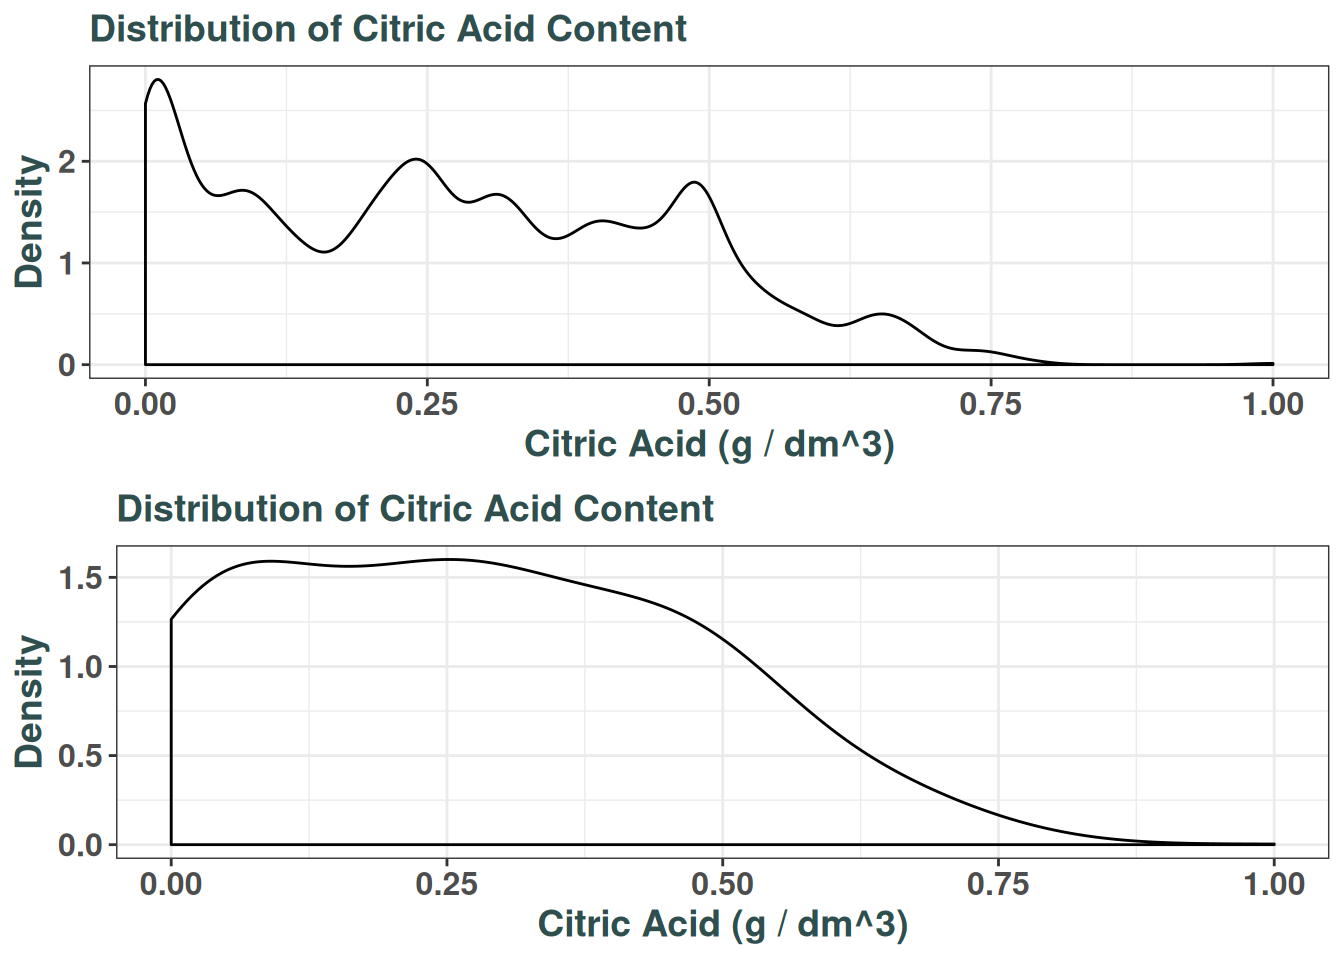
\includegraphics{Homework02_files/figure-latex/unnamed-chunk-5-1.pdf}

\begin{enumerate}
\def\labelenumi{\alph{enumi}.}
\setcounter{enumi}{3}
\item
  (BONUS: 1 point) Remove the ugly \texttt{factor(1)} from the x-axis
  label, without changing the rest of the graphic.
\item
  (BONUS: 1 point) Remove the tick on the x-axis.
\end{enumerate}

\begin{center}\rule{0.5\linewidth}{\linethickness}\end{center}

\begin{center}\rule{0.5\linewidth}{\linethickness}\end{center}

\hypertarget{problem-5}{%
\section{Problem 5}\label{problem-5}}

\textbf{Rose Diagrams}:

\begin{enumerate}
\def\labelenumi{\alph{enumi}.}
\item
  (4 points) Re-create the graph from Problem 3, but use a rose diagram.
  Be sure to correctly label the axes, if necessary. Include an
  appropriate title.
\item
  (3 points) In a rose diagram, what is the radius of each rose petal
  proportional to? What does the angle associated with each rose petal
  correspond to (if anything)? What is the area of each rose petal
  proportaional to?
\end{enumerate}

\begin{center}\rule{0.5\linewidth}{\linethickness}\end{center}

\begin{center}\rule{0.5\linewidth}{\linethickness}\end{center}

\hypertarget{problem-6}{%
\section{Problem 6}\label{problem-6}}

\textbf{Pie Charts}:

To create a pie chart, use a similar technique to what you used to
create a spine chart in Problem 4 (hint: check the argument
\texttt{theta} of the function \texttt{coord\_polar}).

\begin{enumerate}
\def\labelenumi{\alph{enumi}.}
\item
  (4 points) Re-create the graph from Problem 3, but use a pie chart. Be
  sure to correctly label the axes, if necessary. Include an appropriate
  title.
\item
  (3 points) In a pie chart, what does the radius of each pie slice
  correspond to (if anything)? What does the angle associated with each
  pie slice correspond to (if anything)?
\item
  (3 points) Summarize the differences between a rose diagram and a pie
  chart in no more than two sentences.
\item
  (10 points) Of the four graphs we used to visualize the
  \texttt{Pclass} variable, which do you prefer? Why? Discuss the
  strengths (if any) and weaknesses (if any) of each.
\end{enumerate}

\begin{center}\rule{0.5\linewidth}{\linethickness}\end{center}

\begin{center}\rule{0.5\linewidth}{\linethickness}\end{center}

\hypertarget{problem-7}{%
\section{Problem 7}\label{problem-7}}

\textbf{Statistical Tests}:

Your friend says to you, ``The passengers were equally likely to belong
to any of the three classes.''

You obviously disagree. You show your friend your graphs from the
previous four problems, but your friend is still unconvinced, and wants
to know if the differences across the classes in your graph are
statistically significant.

(5 points) What kind of statistical test could you use to show that the
passengers are not equally likely to belong to any of the three classes?
(think back to your earlier statistics classes)

(BONUS: 2 points) What statistical test would you use to answer the
question whether a passenger's class was associated with a passenger's
survival rate?

\begin{center}\rule{0.5\linewidth}{\linethickness}\end{center}

\begin{center}\rule{0.5\linewidth}{\linethickness}\end{center}

\hypertarget{problem-8}{%
\section{Problem 8}\label{problem-8}}

(3 points each)

\textbf{Facetting}:

``Facetting'' refers to the process of partitioning the original data
according to some categorical variable, then creating the same graphic
once for each subset. The resulting graphs are typically displayed in a
grid, where each graph is a single ``facet'' of the full graphic.

This is a popular way to show how the features of the variable(s) being
displayed in a particular graphic can change depending on some other
variable.

With base-\texttt{R} graphics, facetting requires you to write a lot of
code -- code to do the subsetting, code to display the graphics, etc.
With \texttt{ggplot()}, facetting is very easy, as we'll see below.

\begin{enumerate}
\def\labelenumi{\alph{enumi}.}
\item
  Recreate the plot from Problem 3, but this time, facet on the
  \texttt{Embarked} variable. To do this, add
  \texttt{+\ facet\_wrap(\textasciitilde{}\ facetting\_variable)} to the
  existing line of code.
\item
  Adjust the \texttt{ncol} or \texttt{nrow} arguments in
  \texttt{facet\_wrap()}. How do they affect the way
  \texttt{facet\_wrap()} places each facet into a grid of graphs?
\item
  Sometimes, it improves our abiliity to compare across graphics if we
  have all the graphs in a single row or column, rather than having the
  plots displayed in multiple rows and columns. Recreate the plot from
  Problem 3, but this time, facet on the \texttt{Parch} variable using
  the \texttt{facet\_grid()} function. To do this, add
  \texttt{+\ facet\_grid(\textasciitilde{}\ facetting\_variable)} to the
  existing line of code.
\item
  Recreate the graph from part (c), but this time, add
  \texttt{+\ facet\_grid(facetting\_variable\ \textasciitilde{}\ .)}
  instead. What changed? Which version do you prefer for this particular
  problem? Why?
\item
  We can actually facet on multiple categorical variables at once. Let's
  try it. Recreate the graph from part (d), but this time, facet on both
  the \texttt{Sex} and \texttt{Survived} variables. To do this, add
  \texttt{+\ facet\_grid(Sex\ \textasciitilde{}\ Survived)}. Interpret
  the graph. \textbf{Although in your answer please don't wildly
  speculate, I encourage you to ask yourself ``What is going on here?''
  and try to relate the graph to your knowledge about the Titanic (this
  will help prepare you for later in the class).}
\item
  Repeat the facetting but this time use \texttt{Sex} and
  \texttt{Parch}. Some of the facets in the graph are empty. Why? (Hint:
  Look at a contingency table of these two variables with
  \texttt{table(titanic\$Parch,\ titanic\$Sex)}.) Briefly interpret
  graph.
\end{enumerate}

\begin{center}\rule{0.5\linewidth}{\linethickness}\end{center}

\begin{center}\rule{0.5\linewidth}{\linethickness}\end{center}


\end{document}
